\consigne{AireFacile1}{AireFacile6} Calculer les aires des figures suivantes.

\begin{minipage}[t]{0.3\textwidth}
    \exo{Calculer}{AireFacile1}

    \begin{figure}[H]
        \centering
        \begin{tikzpicture}
            \draw (0,0)--(3,0) node[midway,above] {4} ;
            \draw (0,0)--(0,-2) node[midway,left] {3} ;
            \draw (0,-2)--(3,-2) ;
            \draw (3,-2)--(3,0) ;
        \end{tikzpicture}
    \end{figure}
\end{minipage}
\hfill
\begin{minipage}[t]{0.3\textwidth}
    \exo{Calculer}{AireFacile2}

    \begin{figure}[H]
        \centering
        \begin{tikzpicture}
            \draw (0,0)--(2,0) node[midway,above,white] {$L$} ;%Pour alignement
            \draw (0,0)--(0,-2)node[midway,left] {7} ;
            \draw (0,-2)--(2,-2) ;
            \draw (2,-2)--(2,0) ;
        \end{tikzpicture}
    \end{figure}
\end{minipage}
\hfill
\begin{minipage}[t]{0.3\textwidth}
    \exo{Calculer}{AireFacile3}

       \begin{figure}[H]
            \centering
            \begin{tikzpicture}[xscale=0.8,yscale=0.9]
                \draw (-1,0)--(2,0) node[midway,above] {5} ;
                \draw (-1,0)--(0,-2);
                \draw[dotted] (1,0)--(1,-2)node[midway,left] {3} ;
                \draw (0,-2)--(3,-2) ;
                \draw (3,-2)--(2,0) ;
            \end{tikzpicture}
        \end{figure}
\end{minipage}


\begin{minipage}[t]{0.3\textwidth}
    \exo{Calculer}{AireFacile4}

    \begin{figure}[H]
        \centering
            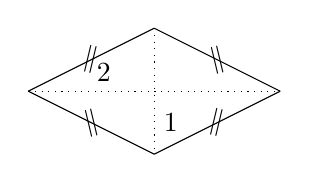
\begin{tikzpicture}[scale=0.8]
                \draw (0,0)--node[sloped, rotate=-40] {$\parallel$}(2,1)  ;%Pour alignement
                \draw (2,1)--node[sloped, rotate=40] {$\parallel$}(4,0);
                \draw [dotted] (0,0)--(4,0) ;
                \node at (1.2,0) [above] {2};
                \node at (2,-0.5) [right] {1};
                \draw [dotted] (2,1)--(2,-1) ;
                \draw (2,-1)--node[sloped, rotate=-40] {$\parallel$}(4,0) ;
                \draw (2,-1)--node[sloped, rotate=40] {$\parallel$}(0,0) ;
            \end{tikzpicture}
        \end{figure}
\end{minipage}
\hfill
\begin{minipage}[t]{0.3\textwidth}
    \exo{Calculer}{AireFacile5}

    \begin{figure}[H]
        \centering
        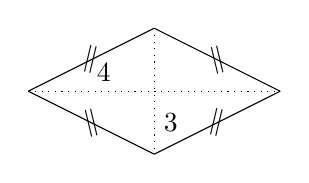
\begin{tikzpicture}[scale=0.8]
            \draw (0,0)--node[sloped, rotate=-40] {$\parallel$}(2,1)  ;%Pour alignement
            \draw (2,1)--node[sloped, rotate=40] {$\parallel$}(4,0);
            \draw [dotted] (0,0)--(4,0) ;
            \node at (1.2,0) [above] {4};
            \node at (2,-0.5) [right] {3};
            \draw [dotted] (2,1)--(2,-1) ;
            \draw (2,-1)--node[sloped, rotate=-40] {$\parallel$}(4,0) ;
            \draw (2,-1)--node[sloped, rotate=40] {$\parallel$}(0,0) ;
        \end{tikzpicture}
    \end{figure}
\end{minipage}
\hfill
\begin{minipage}[t]{0.3\textwidth}
    \exo{Calculer}{AireFacile6}

       \begin{figure}[H]
            \centering
            \begin{tikzpicture}[xscale=0.8,yscale=0.9]
                \draw (-1,0)--(2,0) node[midway,above] {6} ;
                \draw (-1,0)--(0,-2);
                \draw[dotted] (1,0)--(1,-2)node[midway,left] {5} ;
                \draw (0,-2)--(3,-2) ;
                \draw (3,-2)--(2,0) ;
            \end{tikzpicture}
        \end{figure}
\end{minipage}